
\begin{figure}[H]
	\centering
	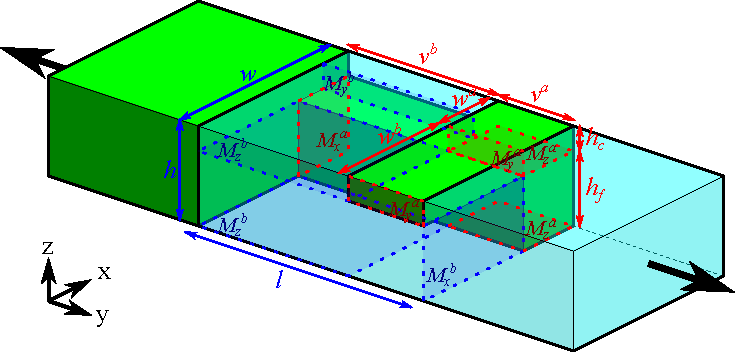
\includegraphics[width=\columnwidth]{sources/method/straight_model_v3.pdf}
	\caption{
		One straight unit cell connecting material $a$ (left) to material $b$ (right).
		Failure can happen along the fingers ($M_x$), along the cross beams ($M_y$) or at the interface between the two ($M_z$) for either material.}
	\label{fig:failure_modes}
\end{figure}


\section{Straight design}





\Cref{fig:failure_modes} shows one cell of the straight structure, along with the design variables and the failure modes.
The optimization then consists of the following:

\begin{align}
	& \max \frac{F}{\left( w^a + w^b \right) \left( h_\text{f} + h_\text{c} \right) } \\
	& \min h_\text{f} h_\text{c} \\
	\text{subject to} & \nonumber \\
	w^m &\ge w_\text{min}^m \\
	v^m &\ge v_\text{min}^m \\
	h_\text{f} &\ge h_\text{min} \\
	h_\text{c} &\ge h_\text{min} \\
	v^a + v^b &\le v_\text{max} \\
	\frac{ F }{ w^m h_\text{f} } &\le \sigma^m_\text{yield} &&\text{ Tension failure } M_x^m \\
	\frac{ 3 F }{ 4 v^m h_\text{c}} &\le \tau^m 			&&\text{ Shear failure } M_y^m \\
	\frac{ 3 F }{ 4 v^m w^m } &\le \tau^m_\text{Z} 			&&\text{ Shear failure } M_z^m \\
	\frac{ 3 F w^b }{ 4 \left( v^a \right)^2 h_\text{c} } &\le \sigma^a_\text{yield}			&&\text{ Bending failure } M_y^a \\
	\frac{ 3 F w^a }{ 4 \left( v^b \right)^2 h_\text{c} } &\le \sigma^b_\text{yield}			&&\text{ Bending failure } M_y^b \\
	& \text{for both materials } && m \in \{a, b\} \nonumber
\end{align}

\iffalse

\paragraph{Monotonicity Analysis}
\begin{align*}
	\min & 1 - \frac{F}{\left( w^a + w^b \right) \left( h_\text{f} + h_\text{c} \right) }
																		&& F^-, w^{a+}, w^{b+},  h_\text{f}^+, h_\text{c}^+\\
	\text{subject to} & \nonumber \\
	1 - \frac{w^m }{w_\text{min}^m} &\le 0    							&& w^{m-} \\
	1 - \frac{v^m }{w_\text{min}^m} &\le 0    							&& v^{m-} \\
	1 - \frac{h_\text{f}}{h_\text{min}} &\le 0 							&& h_\text{f}^- \\
	1 - \frac{h_\text{c}}{h_\text{min}} &\le 0 							&& h_\text{c}^- \\
	\frac{v^a + v^b}{ v_\text{max} }  - 1&\le 0 						&& v^{a+}, v^{b+} \\
	\frac{ F }{ w^m h_\text{f} \sigma^m_\text{yield} } - 1&\le 0 		&& F^+, w^{m-}, h_\text{f}^- \\
	\frac{ 2 F }{ 3 v^m h_\text{c} \tau^m } - 1 &\le 0 					&& F^+, v^{m-}, h_\text{c}^- \\
	\frac{ 2 F }{ 3 v^m w^m \tau^m_\text{Z} } - 1 &\le 0 					&& F^+, v^{m-}, w^{m-} \\
	\nonumber \\
	F^m &= \sigma^m w^m h_\text{f} \\
	\dots \\
	& \text{for both materials } m \in \{a, b\}
\end{align*}
\fi


This looks like a multi-objective optimization problem, but without the second objective the problem is under-constrained.
Adding the second objective actually means there's one unique solution - rather counter-intuitively.

The $v^m$ variables don't figure in the objective, but they do appear in the constraints and therefore are also subject to the optimization.

We should be able to find analytical solution(s), depending on the size of $v_\text{max}$ w.r.t. the other constraints.

Possible extensions:
\begin{itemize}
	\item Consider multiple repetitions of the cell in the loading direction.
	\item Consider tensile load in Z direction.
	\item Consider FEM model.
\end{itemize}

\iffalse
Formula is given by this? :
% from https://skyciv.com/docs/tutorials/beam-tutorials/bending-moment-equations/
\begin{align*}
	\sigma_\text{bend} &= \frac{M r}{I} \\
	&= \frac{M \nicefrac12 v}{I} \\
	M_\text{max} &= \frac{v L}{12} \text{ for distributed force and fixed sides} 
\end{align*}
\fi

